% !TEX root = handbook-physics.tex
% !TEX TS-program = pdflatex
% !TEX encoding = UTF-8 Unicode




\chapter{Elements Of Quantum Mechanics}
\label{ch-38}
\zhtitle{量子力学基础}

\section[Wave-Particle Dualism]{Wave-Particle Dualism of the Properties of Particles of Matter}
\label{sec-38.1} 
\zhtitle{物质粒子性质的波粒二象性}

\subsection{}\label{38.1.1} Quantum mechanics\sidenote{Also called \redem{wave mechanics} in its early stages of development.} deals with the physics of atoms,
molecules and their associations, crystals in particular, as well ;is atomic nuclei and elementary particles. Objects of the microcosm studied by quantum mechanics have linear dimensions of the order of \num{d-6} to \SI{d-13}{\centi\meter}. If the particles travel at velocities
$v \ll c$, where $c$ is the velocity of light in free space, non-relativistic quantum mechanics is applied; at $v \lesssim c$, relativistic quantum mechanics is resorted to.\sidenote{Information on relativistic quantum mechanics is beyond the scope of the present handbook. Wherever applied, the term quantum mechanics refers to non-relativistic quantum mechanics.}
\zhpar{量子力学研究原子、分子及其结合体（特别是晶体）、原子核和基本粒子的规律。量子力学所研究的微观客体，其线度约为 \num{d-6} 至 \SI{d-13}{\centi\meter}。若粒子的运动速度满足 $v \ll c$（其中 $c$ 为真空中的光速），则应用非相对论量子力学；当 $v \lesssim c$ 时，则需采用相对论量子力学。}
\zhpar{注：在量子力学发展的早期阶段，它也称为\redem{波动力学}。}
\zhpar{注：有关相对论量子力学的内容超出了本手册的范围。无论在何处使用，术语“量子力学”均指非相对论量子力学。}

\subsection{}\label{38.1.2} Quantum mechanics is based on Plancks concepts concerning the discrete nature of changes in the energy of atoms \ssect{36.3.2}, Einstein's ideas on photons \ssect{37.1.4}, and data on the quantum nature of certain physical quantities (momentum and energy, for instance) that characterize, under definite conditions, the states of particles of the microcosm.
\zhpar{量子力学建立在以下概念之上：普朗克关于原子能量变化具有不连续性的概念（\ssect{36.3.2}）、爱因斯坦关于光子的思想（\ssect{37.1.4}），以及关于某些物理量（例如动量和能量）具有量子性质的数据。这些物理量在一定条件下表征微观粒子的状态。}

\subsection{}\label{38.1.3} The basic concept of quantum mechanics is that the wave-particle dualism of properties, established for light \ssect{37.4.1}, is of a universal nature. It should manifest itself for any particles
having a momentum $p$. All particles with the finite momentum
$p$ possess wave properties and their motion is accompanied
by a certain wave process.
\zhpar{量子力学的基本概念是：光已经确立的波粒二象性（\ssect{37.4.1}）具有普遍性。它应当表现在任何具有动量 $p$ 的粒子上。所有具有有限动量 $p$ 的粒子都具有波动性质，其运动伴随着某种波动过程。}

\subsection{}\label{38.1.4} The de Broglie formula establishes the dependence of the wavelength associated with a moving particle of matter on the momentum p of the particle. Thus
\zhpar{德布罗意公式给出了与运动物质粒子相联系的波长同粒子动量 $p$ 之间的关系。由此得到：}
\begin{equation*}%
\lambda = \frac{h}{p} = \frac{h}{mv},
\end{equation*}
where $m$ is the mass of the particle, $v$ is its velocity, and $h$ is Planck's constant (Appendix~II). The waves mentioned here are called \redem{de Broglie}, or \redem{matter waves}.
\zhpar{式中 $m$ 为粒子的质量，$v$ 为其速度，$h$ 为普朗克常量（见附录 II）。这里所说的波称为\redem{德布罗意波}，或\redem{物质波}。}

Another form of the de Broglie formula is
\zhpar{德布罗意公式的另一种形式为：}
\begin{equation*}%
\vb{p} = \frac{h}{2\pi} \vb{k} = \hbar \vb{k},
\end{equation*}
where $\vb{k} = 2\pi \vu{n}/\lambda$ is the wave vector, whose magnitude $k = = 2\pi/\lambda$ is the wavenumber, i.e. the number of wavelengths per $2\pi$ units of length, $\vu{n}$ is a unit vector in the direction of wave propagation, and $\hbar = h/2\pi = \SI{1.05d-34}{\joule\second}$.
\zhpar{式中 $\vb{k} = 2\pi \vu{n}/\lambda$ 为波矢，其大小 $k = = 2\pi/\lambda$ 即波数，表示单位长度为 $2\pi$ 时所含的波长数；$\vu{n}$ 为沿波传播方向的单位矢量；$\hbar = h/2\pi = \SI{1.05d-34}{\joule\second}$。}

\subsection{}\label{38.1.5} The de Broglie wavelength for a particle of mass $m$, having the kinetic energy $E_{k}$ \ssect{3.2.1}, is
\zhpar{质量为 $m$、动能为 $E_{k}$（\ssect{3.2.1}）的粒子，其德布罗意波长为：}
\begin{equation*}%
\lambda = \frac{h}{\sqrt{2m E_{k}}}.
\end{equation*}
In particular, for an electron accelerated in an electric field
with a potential difference of $\Delta V$ volts \ssect{16.2.7},
\zhpar{特别地，对于在电势差为 $\Delta V$ 伏特（\ssect{16.2.7}）的电场中加速的电子，其德布罗意波长为：}
\begin{equation*}%
\lambda = \frac{12.25}{\sqrt{\Delta V}} \si{\angstrom}.
\end{equation*}

\subsection{}\label{38.1.6} The de Broglie formula is confirmed by experiments in the scattering of electrons and other particles by crystals and in the passage of particles through matter. An indication of the wave process in all such experiments is the diffraction pattern observed, showing the distribution of the electrons (or other particles) in the particle detecting devices.
\zhpar{德布罗意公式已为电子及其他粒子在晶体上的散射实验以及粒子穿过物质的实验所证实。在所有这类实验中，波动过程的标志是所观察到的衍射图样，它显示了电子（或其他粒子）在粒子探测装置中的分布。}

No wave properties are manifested by macroscopic bodies. The
de Broglie wavelengths for such bodies are so short that it
proves impossible to detect any wave properties.
\zhpar{宏观物体不表现出任何波动性质。这类物体的德布罗意波长极短，以致无法探测到其任何波动性质。}

\subsection{}\label{38.1.7} The phase velocity \ssect{30.2.10} of de Broglie waves is
\zhpar{德布罗意波的相速度为：}
\begin{equation*}%
v_{ph} = \frac{\omega}{k} = \frac{c^{2}}{v} = \frac{c^{2}}{h} m \lambda,
\end{equation*}
where $m$ is the mass of the particle, $v$ is its velocity, and $\lambda$ is the de Broglie wavelength. Since $c > v$, the phase velocity of de Broglie waves is greater than the velocity of light in free space. 
\zhpar{式中 $m$ 为粒子的质量，$v$ 为其速度，$\lambda$ 为德布罗意波长。由于 $c > v$，德布罗意波的相速度大于真空中的光速。}

The dependence of the phase velocity of de Broglie waves on the wavelength indicates that these waves undergo dispersion \ssect{30.3.8}. The group velocity \ssect{30.4.3} of de Broglie waves is equal to the particle velocity $v$. Thus
\zhpar{德布罗意波的相速度随波长而变化，这表明这些波会发生色散（\ssect{30.3.8}）。德布罗意波的群速度（\ssect{30.4.3}）等于粒子的速度 $v$，即：}
\begin{equation*}%
u = \dv{\omega}{k} = v.
\end{equation*}

\tabl{tab-38.1} compares the particle and wave properties of particles of mass $m$, travelling at the velocity $v$.
\zhpar{\tabl{tab-38.1}比较了质量为 $m$、以速度 $v$ 运动的粒子的粒子性质与波动性质。}

\begin{table}
\begin{small}
\begin{center}
\begin{tabular}{p{2cm}p{5cm}}
\toprule
\textbf{Particle like properties} & \textbf{Wavelike properties} \\
\midrule
Velocity $v$ & De Broglie wavelength \newline $\lambda = \dfrac{h}{p} = \dfrac{h}{mv} $\\
Momentum $p = mv$ &  De Broglie wave frequency \newline  $\nu = \dfrac{E}{h} = \dfrac{mc^{2}}{h} $ \\
Energy $E = mc^{2}$ & Group velocity of de Broglie waves \newline  $u = v$ \newline
Phase velocity of de Broglie waves \newline  $v_{ph} = \dfrac{c^{2}}{v}$\\
\bottomrule
\end{tabular}
\end{center}
\end{small}
\sidecaption{Table comparing the particle and wave properties. \zhcap{比较粒子性质与波动性质的表。}\label{tab-38.1}}
\end{table}


\subsection{}\label{38.1.8} Besides the de Broglie formula, it is assumed in quantum mechanics that the following relation exists between the total energy $E$ of a particle and the frequency $\nu$ of its de Broglie wave:
\zhpar{除德布罗意公式外，量子力学还假定：粒子的总能量 $E$ 与其德布罗意波频率 $\nu$ 之间存在如下关系：}
\begin{equation*}%
E = h \nu = \hbar \omega,
\end{equation*}
where $\omega = 2\pi \nu$ is the angular frequency \ssect{28.1.2} and $\hbar = h/2\pi$ \ssect{38.1.4}.
\zhpar{式中 $\omega = 2\pi \nu$ 为角频率（\ssect{28.1.2}），$\hbar = h/2\pi$（见\ssect{38.1.4}）。}

\subsection{}\label{38.1.9} De Broglie waves are of a specific nature having no analogies among the waves dealt with in classical physics. The square of the magnitude of the de Broglie wave's amplitude at a given point is a measure of the probability that the particle is to be found at this point (this is the \redem{probability, or statistical, meaning of de Broglie waves}). 
\zhpar{德布罗意波具有特殊的性质，在经典物理学所研究的波中找不到与之类似的波。德布罗意波在某点的振幅模的平方，是粒子在该点被发现的概率的量度（这就是\redem{德布罗意波的概率意义，或统计意义}）。}

The diffraction patterns, observed in the experiments mentioned in Section~\ssect{38.1.6}, are an indication of statistical laws. According to these laws the particles, reach definite places in the receivers, these being the places where the intensity \ssect{30.3.6} of the de Broglie wave is found to be
highest. No particles are observed at the places where, according to the statistical interpretation, the square of the magnitude of the ``probability wave'' amplitude becomes zero.
\zhpar{在\ssect{38.1.6}所述实验中观察到的衍射图样，表明了统计规律。根据这些规律，粒子到达接收器中的一定位置，这些位置正是德布罗意波强度（\ssect{30.3.6}）最大之处。按照统计解释，在“概率波”振幅模的平方为零的地方，观察不到任何粒子。}

\section{Schr\"odinger Wave Equation}
\label{sec-38.2} 
\zhtitle{薛定谔波动方程}


\subsection{}\label{38.2.1} The position of a particle in space at a given instant of time is determined in quantum mechanics by specifying its \redem{Schr\"odinger wave function} (also called the \redem{psi function} or the \redem{probability amplitude})  $\psi (x,\, y,\, z,\, t)$. The probability $\dd w$ that the particle is within the element $\dd V$ of volume is proportional to $\abs{\psi}^{2}$ and to the element $\dd V$ of volume. Thus
\zhpar{在量子力学中，粒子在给定时刻的空间位置由其\redem{薛定谔波函数}（亦称\redem{$\psi$ 函数}或\redem{概率幅}）$\psi (x,\, y,\, z,\, t)$ 确定。粒子处于体积元 $\dd V$ 内的概率 $\dd w$ 正比于 $\abs{\psi}^{2}$ 以及体积元 $\dd V$。即：}
\begin{equation*}%
\dd w = \abs{\psi}^{2}\, \dd V,
\end{equation*}
where $\abs{\psi}^{2}$ is the square of the magnitude of the psi function: $\abs{\psi}^{2} = \psi \psi^{*}$. Here $\psi^{*}$ is a function that is the complex conjugate of $\psi$. The quantity $\abs{\psi}^{2}$ is the \redem{probability density} $\abs{\psi}^{2} = \dv*{w}{V} = \rho$ and specifies the probability of the particle occupying the given point in space. The intensity of the de Broglie wave is determined by the quantity $\abs{\psi}^{2}$.
\zhpar{式中 $\abs{\psi}^{2}$ 为 $\psi$ 函数模的平方，$\abs{\psi}^{2} = \psi \psi^{*}$，其中 $\psi^{*}$ 为 $\psi$ 的复共轭函数。量 $\abs{\psi}^{2}$ 称为\redem{概率密度} $\abs{\psi}^{2} = \dv*{w}{V} = \rho$，它确定粒子占据空间给定点的概率。德布罗意波的强度由量 $\abs{\psi}^{2}$ 决定。}

\subsection{}\label{38.2.2} Following from the definition of the psi function is the \redem{normalization condition for probabilities}:
\zhpar{由 $\psi$ 函数的定义得出的是\redem{概率归一化条件}：}
\begin{equation*}%
 \iiint \abs{\psi}^{2}\, \dd V = 1,
\end{equation*}
in which the triple integral with respect to volume is calculated along the coordinates $x$, $y$ and $z$, from $-\infty$ to $+\infty$, i.e. throughout the whole infinite space. The normalization condition indicates that it is a certain event that the particle is some­ where in space and the probability of this event should be unity.
\zhpar{式中三重积分沿坐标 $x$、$y$、$z$ 从 $-\infty$ 积分到 $+\infty$，即对整个无限空间积分。归一化条件表明：粒子必定处于空间中的某个位置，这是一个必然事件，其概率应等于 1。}

\subsection{}\label{38.2.3} The wave function $\psi(x, \,y,\, z,\, t)$ is the main characteristic of the state of micro-objects (atoms, molecules and elementary particles). This function is made use of to calculate the average value of some physical quantity $L$ that characterizes the object which is in the state described by the wave function $\psi$. Thus
\zhpar{波函数 $\psi(x, \,y,\, z,\, t)$ 是微观客体（原子、分子和基本粒子）状态的主要特征量。利用它可以计算处于波函数 $\psi$ 所描述状态的客体的某一物理量 $L$ 的平均值，即：}
\begin{equation*}%
\expval{L} = \iiint L \abs{\psi}^{2}\, \dd x \dd y \dd z,
\end{equation*}
where $\expval{L}$ is the average value of $L$ and integration is carried out as indicated in Section~\ssect{38.2.2}.
\zhpar{式中 $\expval{L}$ 为 $L$ 的平均值，积分按\ssect{38.2.2}中所示进行。}

\subsection{}\label{38.2.4} The fundamental differential equation of quantum mechanics\sidenote{See the second footnote to \ssect{38.1.1}.}, concerning the wave function $\psi(x, \,y,\, z,\, t)$ is called the \redem{Schr\"odinger time-dependent wave equation}. It determines the psi function for microparticles in a field of force with the potential energy $U (x, \,y,\, z,\, t)$ \ssect{3.3.1} at the velocity $v \ll c$, where $c$ is the velocity of light in free space. The Schr\"odinger equation is of the form
\zhpar{量子力学的基本微分方程是关于波函数 $\psi(x, \,y,\, z,\, t)$ 的方程，称为\redem{薛定谔含时波动方程}。它决定了在势能为 $U (x, \,y,\, z,\, t)$（\ssect{3.3.1}）的力场中、速度 $v \ll c$（其中 $c$ 为真空中的光速）运动的微观粒子的 $\psi$ 函数。薛定谔方程的形式为：}
\zhpar{注：参见\ssect{38.1.1}中的第二条脚注。}
\begin{equation*}%
i \hbar \pdv{\psi}{t} = -\frac{\hbar^{2}}{2m} \laplacian \psi + U(x, \,y,\, z,\, t) \psi,
\end{equation*}
where $\laplacian$ is the Laplace operator, $m$ is the mass of the particle, $\hbar = h/2\pi$, $h$ is Planck's constant, and $i = \sqrt{-1}$.
\zhpar{式中 $\laplacian$ 为拉普拉斯算符，$m$ 为粒子的质量，$\hbar = h/2\pi$，$h$ 为普朗克常量，$i = \sqrt{-1}$。}

The Schr\"odinger equation is supplemented by the following
conditions that are imposed on the psi function:
\zhpar{薛定谔方程还须满足对 $\psi$ 函数施加的下列条件：}
\begin{enumerate}[label=(\alph*),noitemsep]
\item the psi function should be finite, single-valued and continuous;
\zhpar{$\psi$ 函数应为有限、单值且连续的；}
\item the partial derivatives $\pdv*{\psi}{x}$, $\pdv*{\psi}{y}$ and $\pdv*{\psi}{z}$ should be continuous;
\zhpar{偏导数 $\pdv*{\psi}{x}$、$\pdv*{\psi}{y}$ 和 $\pdv*{\psi}{z}$ 应连续；}
\item the function $\abs{\psi}^{2}$ should be integrable, i.e. the integral $\iiint^{+\infty}_{-\infty} L \abs{\psi}^{2}\, \dd V $ should be finite. In the simplest cases, this condition is reduced to the normalization of probabilities \ssect{38.2.2}.
\zhpar{函数 $\abs{\psi}^{2}$ 应为可积的，即积分 $\iiint^{+\infty}_{-\infty} L \abs{\psi}^{2}\, \dd V $ 应为有限值。在最简单的情形下，此条件归结为概率的归一化（\ssect{38.2.2}）。}
\end{enumerate}

\subsection{}\label{38.2.5} In the case when the psi function is time-independent, i.e. $\psi = \psi(x,\, y,\, z)$, it satisfies the Schr\"odinger steady-state equation:
\zhpar{当 $\psi$ 函数不含时间，即 $\psi = \psi(x,\, y,\, z)$ 时，它满足薛定谔定态方程：}
\begin{equation*}%
\laplacian \psi + \frac{2m}{\hbar^{2}} (E - U) \psi = 0,
\end{equation*}
where $E$ is the total energy of the particle. The remaining notation is given in Section~\ssect{38.2.4}. The psi functions satisfying the Schr\"odinger equation for the given form of $U = U (x,\, y,\, z)$ are called \redem{eigenfunctions}. They exist only at definite values of $E$, called the \redem{eigenvalues of the energy}. The whole set of eigenvalues of $E$ forms the \redem{energy spectrum of the particle}. If $U$ is a monotonic function and $U \to 0$ at infinity, then in the region $E < 0$, the eigenvalues of the energy form a \redem{discrete spectrum}. The most important problem of quantum mechanics is to find the eigenvalues and eigenfunctions of particles (or systems of particles).
\zhpar{式中 $E$ 为粒子的总能量，其余符号的含义见\ssect{38.2.4}。满足给定形式 $U = U (x,\, y,\, z)$ 的薛定谔方程的 $\psi$ 函数称为\redem{本征函数}。它们只在 $E$ 取确定值时存在，这些确定值称为\redem{能量本征值}。全部本征值构成\redem{粒子的能谱}。若 $U$ 为单调函数，且当趋于无穷远时 $U \to 0$，则在 $E < 0$ 的区域内，能量本征值构成\redem{分立谱}。量子力学中最重要的问题，就是求出粒子（或粒子体系）的本征值和本征函数。}

\subsection{}\label{38.2.6} Schr\"odinger's time-dependent equation has the solution:
\zhpar{薛定谔含时方程的解为：}
\begin{equation*}%
\psi (x,\, y,\, z,\, t ) = \psi (x,\, y,\, z) \exp \left( -\frac{iEt}{\hbar} \right).
\end{equation*}
The state of the particle at the given instant of time is described by a periodic function of time with the angular frequency $\omega = E/\hbar$, determined by the total energy $E$ of the particle. This corresponds to the relation between the total energy $E$ of the particle and the de Broglie wave frequency \ssect{38.1.8}.
\zhpar{粒子在给定时刻的状态由一个随时间做周期变化的函数描述，其角频率为 $\omega = E/\hbar$，由粒子的总能量 $E$ 决定。这与粒子总能量 $E$ 和德布罗意波频率之间的关系相一致（\ssect{38.1.8}）。}

If a particle is in a definite energy state with the energy $E = \text{const.}$, the probability $\dd w$ of finding it in the element $\dd V$ of volume is independent of time. Thus
\zhpar{若粒子处于能量为 $E = \text{const.}$ 的确定能态，则其出现在体积元 $\dd V$ 内的概率 $\dd w$ 与时间无关，即：}
\begin{equation*}%
\dd w = \abs{\psi}^{2} \dd V = \psi \psi^{*} \dd V.
\end{equation*}
This is said to be the \redem{steady state} of the particle. An atom in the steady state has constant energy and does not radiate electromagnetic waves \ssect{39.1.7}.
\zhpar{这种状态称为粒子的\redem{定态}。处于定态的原子具有恒定的能量，且不辐射电磁波（\ssect{39.1.7}）。}

\section{Motion of a Free Particle}
\label{sec-38.3} 
\zhtitle{自由粒子的运动}

\subsection{}\label{38.3.1} In free motion of a particle $(U = 0)$, its total energy $E$ coincides with its kinetic energy. If the $OX$ axis is taken along vector $\vb{v}$ of the particle's velocity $(\vb{v} = \text{const.})$, Schr\"odinger's steady-state equation \ssect{38.2.4} has the following solution:
\zhpar{在自由运动（$U = 0$）中，粒子的总能量 $E$ 与其动能相等。取 $OX$ 轴沿粒子速度 $\vb{v}$ 的方向（$\vb{v} = \text{const.}$），薛定谔定态方程（\ssect{38.2.4}）的解为：}
\begin{equation*}%
\psi = A \exp \left(- \frac{i \sqrt{2mE} x}{\hbar} \right) + B \exp \left(\frac{i \sqrt{2mE} x}{\hbar} \right),
\end{equation*}
where $m$ is the mass of the particle, $\hbar = h/2\pi$, $h$ is Planck's constant, and $A$ and $B$ are certain constants. The Schr\"odinger time-dependent equation \ssect{38.2.4} has, in this case, the solution
\zhpar{式中 $m$ 为粒子的质量，$\hbar = h/2\pi$，$h$ 为普朗克常量，$A$ 和 $B$ 为待定常量。在这种情形下，薛定谔含时方程（\ssect{38.2.4}）的解为：}
\begin{equation*}%
\begin{split}
\psi(x,\, y,\, z,\, t) & = A \exp \left(-i \frac{E}{h}t -\frac{\sqrt{2mE} x}{\hbar} \right) \\
& + B \exp \left( i\frac{E}{h}t +\frac{\sqrt{2mE} x}{\hbar} \right),
\end{split}
\end{equation*}
which is the superposition of two plane monochromatic waves
\ssect{31.1.6} of equal frequency $\omega = E/\hbar$, propagating, one in the positive direction of the $OX$ axis with the amplitude $A$ and the other in the opposite direction with the amplitude $B$.
\zhpar{该解是两个频率相同（$\omega = E/\hbar$）的平面单色波的叠加：一个沿 $OX$ 轴正方向传播，振幅为 $A$；另一个沿相反方向传播，振幅为 $B$。}

\subsection{}\label{38.3.2} In quantum mechanics a free particle is described by a plane monochromatic de Broglie wave with the wavenumber $k$ \ssect{38.1.4}:
\zhpar{在量子力学中，自由粒子用波数为 $k$（\ssect{38.1.4}）的平面单色德布罗意波描述：}
\begin{equation*}%
k = \frac{1}{\hbar} \sqrt{2mE}.
\end{equation*}
The probability of finding the particle at any point in space is constant. For waves propagating along the positive direction of the $OX$ axis,
\zhpar{粒子在空间任一点被发现的概率都是常数。对于沿 $OX$ 轴正方向传播的波，有：}
\begin{equation*}%
\abs{\psi}^{2} =  \psi \psi^{*} = \abs{A}^{2}.
\end{equation*}

\section{A Particle in a One-Dimensional Infinitely
Deep Potential Well}
\label{sec-38.4} 
\zhtitle{一维无限深势阱中的粒子}

\subsection{}\label{38.4.1} A \redem{potential well} is a region of space in which the potential energy $U$ of a particle is less than a certain value $U_{max}$. In particular, at $U = U (x)$ and $U_{max} = \infty$, there is a one dimensional potential well of infinite depth. If the potential energy of the particle outside and inside the potential well has the following values (\figr{fig-38-01}:
\zhpar{若粒子在势阱内、外的势能取如下数值（见\figr{fig-38-01}）：}
\begin{align*}%
U & = 0 \text{ at } 0 \leqslant x \leqslant L,\\
U & = \infty \text{ at } x \leqslant 0 \qand  x \geqslant L,
\end{align*}
the well has a ``flat bottom''.
\zhpar{该势阱具有“平底”。}


\begin{marginfigure}%[-3cm] 
\centering
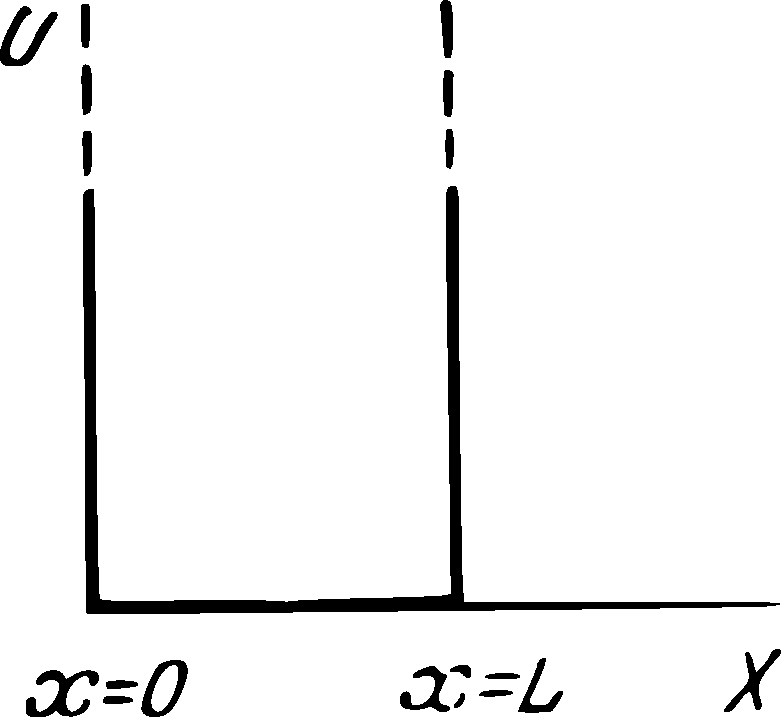
\includegraphics[width=0.7\textwidth]{figs/ch-38/fig-38-01.pdf}
\sidecaption{A one dimensional potential well.\zhcap{一维势阱。}\label{fig-38-01}}
\end{marginfigure}

The motion of collectivized electrons in a metal is dealt with
in classical electronic theory as motion in a potential well,
the potential energy of the electron outside the metal equalling zero, and that inside the metal being negative and numerically equal to the work function of the metal (energy required to remove an electron from the metal) \ssect{41.11.1}. The potential well illustrated in \figr{fig-38-01} is simpler than the real potential well of electrons in a metal.
\zhpar{金属中共有化电子的运动，在经典电子理论中被视为势阱中的运动：电子在金属外的势能为零，在金属内的势能为负值，其数值等于金属的逸出功（即将电子从金属中移出所需的能量，见\ssect{41.11.1}）。\figr{fig-38-01}中所示的势阱比金属中电子的实际势阱要简单。}

\subsection{}\label{38.4.2} The Schr\"odinger steady-state
equation (38.2.5) for particles in a potential well, considered in the preceding subsection, is of the form
\zhpar{对于上一小节所考虑的势阱中的粒子，薛定谔定态方程（38.2.5）的形式为：}
\begin{equation*}%
\dv[2]{\psi}{x} + \frac{2m}{\hbar^{2}} E \psi = 0,
\end{equation*}
at boundary conditions $\psi (0) = \psi (L) = 0$, which indicate that $\psi = 0$ and $\abs{\psi}^{2} = 0$ outside the region $0 \leqslant x \leqslant L$, i.e. that the probability of finding the particle outside the potential well is zero.
\zhpar{边界条件 $\psi (0) = \psi (L) = 0$ 表明，在区域 $0 \leqslant x \leqslant L$ 之外 $\psi = 0$ 且 $\abs{\psi}^{2} = 0$，即粒子出现在势阱之外的概率为零。}

The solution of the Schr\"odinger equation is
\zhpar{薛定谔方程的解为：}
\begin{equation*}%
\psi(x) = A \cos k x  + B \sin kx,
\end{equation*}
where $A$ and $B$ are constants, and $k = \sqrt{2mE/\hbar}$ is the wavenumber \ssect{38.1.4}. It follows from the boundary conditions that $A = 0$, $B \neq 0$ and $\sin kL = 0$, i.e. the wavenumber can assume a set of discrete values that comply with the requirement: $knL = n \pi$, where $n = 1, \,2, \,3, \ldots{}$
\zhpar{式中 $A$ 和 $B$ 为常量，$k = \sqrt{2mE/\hbar}$ 为波数（\ssect{38.1.4}）。由边界条件可知 $A = 0$，$B \neq 0$，且 $\sin kL = 0$，即波数只能取满足下列要求的一组分立值：$knL = n \pi$，其中 $n = 1,\, 2,\, 3,\, \ldots{}$。}

The last equation means that
\zhpar{上式表示：}
\begin{equation*}%
\frac{2\pi}{\lambda_{n}} = \frac{\pi n}{L} \qor \lambda_{n} = \frac{2L}{n}. 
\end{equation*}
A whole number of de Broglie half-waves should fit into the length of the potential well.
\zhpar{即势阱的宽度内应恰好容纳整数个德布罗意半波。}

\subsection{}\label{38.4.3} Physical quantities that can have only definite discrete values are said to be \redem{quantized (quantized physical quantities)}. The eigenvalues of the energy $E_{n}$ of a particle in a one-dimensional infinitely deep potential well,
\zhpar{只能取确定分立值的物理量称为\redem{量子化物理量}。一维无限深势阱中粒子的能量本征值 $E_{n}$ 为：}
\begin{equation*}%
E_{n} = \frac{n^{2}\pi^{2} \hbar^{2}}{2mL^{2}} \quad (n = 1,\, 2, \, \ldots{}). 
\end{equation*}
comprise a discrete set of energy values that are quantized (see also Section \ssect{38.2.5}).
\zhpar{这些能量本征值构成一组分立的量子化能量值（另见\ssect{38.2.5}）。}

The quantized values of $E_{n}$ are called \redem{energy levels}, and the numbers $n$, determining the energy levels of a particle in a potential well, are called \redem{quantum numbers}.
\zhpar{量子化的能量值 $E_{n}$ 称为\redem{能级}，决定粒子在势阱中能级的数 $n$ 称为\redem{量子数}。}

\subsection{}\label{38.4.4} At large quantum numbers $( n \gg 1)$, the energy levels of a particle in a potential well become relatively closer to one another. The relation $\Delta E/E_{n} \approx 2/n \ll 1$, where $\Delta E = E_{n+1} -
- E_{n} = (2n +1) n^{2}\hbar^{2}/2mL^{2}$. The inequality $\Delta E \ll E_{n}$ at $n \gg 1$ indicates that the quantization of energy at large quantum numbers yields results close to those obtained in classical physics: the energy levels become \redem{quasi-continuous} (quasi-continuous energy levels at $n \gg 1$).
\zhpar{当量子数 $n \gg 1$ 时，粒子在势阱中的能级彼此相对靠近。关系式 $\Delta E/E_{n} \approx 2/n \ll 1$ 中，$\Delta E = E_{n+1} - E_{n} = (2n +1) n^{2}\hbar^{2}/2mL^{2}$。当 $n \gg 1$ 时 $\Delta E \ll E_{n}$，这表明在大量子数情形下，能量量子化所得结果接近经典物理的结果：能级变为\redem{准连续}的（即当 $n \gg 1$ 时为准连续能级）。}

\redem{Bohr's correspondence principle} states that at high quantum numbers the conclusions and results obtained in quantum mechanics should correspond to those of classical mechanics.
\zhpar{\redem{玻尔对应原理}指出：在大量子数情形下，量子力学中得出的结论和结果应当与经典力学的结论和结果相对应。}

A more general statement of the correspondence principle is
that between any theory developed from a classical one and the
initial classical theory there must be a regular relationship:
in definite limiting cases, the new theory must go over into the old one. For example, the formulas of kinematics and dynamics of the special theory of relativity become the formulas of Newton's mechanics at velocities where $(v/c)^{2} \ll 1$ \ssect{5.3.4}. Geometrical optics is a limiting case of wave optics if the wavelength can be neglected $(\lambda \to 0)$.
\zhpar{对应原理的更一般表述为：任何由经典理论发展而来的新理论，与原有的经典理论之间都必须存在确定的联系：在一定的极限情形下，新理论必须过渡到旧理论。例如，狭义相对论的运动学和动力学公式，当速度满足 $(v/c)^{2} \ll 1$ 时，变为牛顿力学的公式（\ssect{5.3.4}）。若波长可以忽略（$\lambda \to 0$），则几何光学是波动光学的极限情形。}

\section{Linear Harmonic Oscillator}
\label{sec-38.5} 
\zhtitle{线性谐振子}


\subsection{}\label{38.5.1} A \redem{linear (one-dimensional) harmonic oscillator} is a particle of mass $m$, vibrating with the natural angular frequency $\omega_{0}$ \ssect{28.1.2} along a certain axis $OX$ due to the action of quasi-elastic
force $F$, which is proportional to the displacement $x$ of
the particle from its equilibrium position. Thus $F = -kx$.
Here $k$ is a factor of the quasi-elastic force, related to $m$ and $\omega_{0}$ by the equation: $k = m\omega^{2}$ \ssect{28.2.3}. The potential energy $U$ of the harmonic oscillator \ssect{28.2.3} is
\zhpar{\redem{线性（一维）谐振子}是指质量为 $m$ 的粒子沿某一轴 $OX$ 振动，其固有角频率为 $\omega_{0}$（\ssect{28.1.2}），振动由与粒子离开平衡位置的位移 $x$ 成正比的准弹性力 $F$ 作用引起。即 $F = -kx$。式中 $k$ 为准弹性力系数，它与 $m$、$\omega_{0}$ 之间的关系为 $k = m\omega^{2}$（\ssect{28.2.3}）。谐振子的势能 $U$（\ssect{28.2.3}）为：}
\begin{equation*}%
U(x) = \frac{kx^{2}}{2}.
\end{equation*}



\subsection{}\label{38.5.2} In classical physics the amplitude \ssect{28.1.3} of small vibration of a harmonic oscillator is determined by the margin of its total energy $E$ (\figr{fig-38-02}). At points $B$ and $A$, with the coordinates $\pm a$, the total energy $E$ is equal to the potential energy:
\zhpar{在经典物理中，微小振动谐振子的振幅（\ssect{28.1.3}）由其总能量 $E$ 的大小决定（见\figr{fig-38-02}）。在坐标为 $\pm a$ 的 $B$、$A$ 两点处，总能量 $E$ 等于势能：}
\begin{marginfigure}%[-3cm] 
\centering
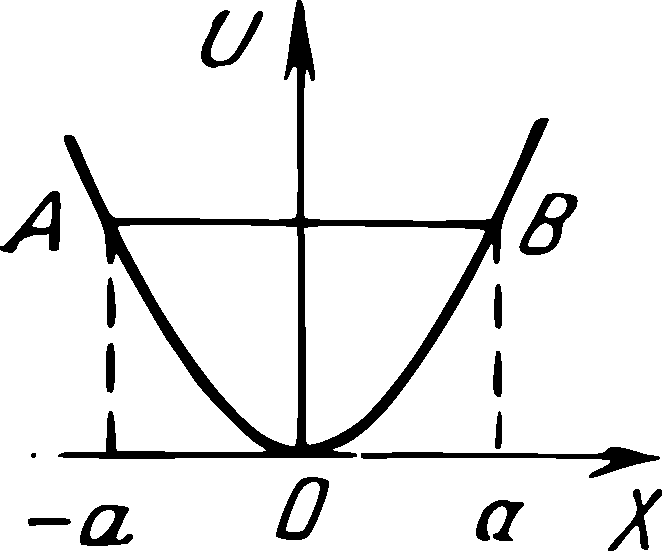
\includegraphics[width=0.7\textwidth]{figs/ch-38/fig-38-02.pdf}
\sidecaption{A linear harmonic oscillator.\zhcap{线性谐振子。}\label{fig-38-02}}
\end{marginfigure}
\begin{equation*}%
E = 	
\begin{cases}
  U(a) \\
    U(-a)
  \end{cases}
\end{equation*}
where $a$ is the amplitude of vibration of the classical harmonic oscillator. Such an oscillator cannot get outside
the limits of the region $(-a, + a)$.
\zhpar{式中 $a$ 为经典谐振子振动的振幅。这种振子不能超出区域 $(-a, + a)$ 的范围。}

\begin{marginfigure}[1cm] 
\centering
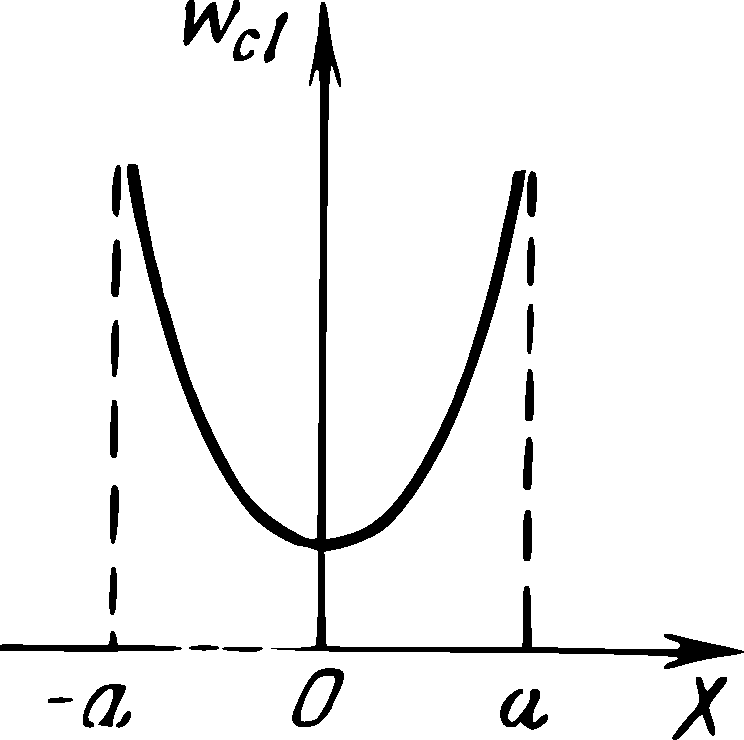
\includegraphics[width=0.7\textwidth]{figs/ch-38/fig-38-03.pdf}
\sidecaption{Classical probability $w_{cl}$ of finding the oscillator in the line segment $x$.\zhcap{谐振子位于线段 $x$ 内的经典概率 $w_{cl}$。}\label{fig-38-03}}
\end{marginfigure}

\subsection{}\label{38.5.3} The probability $w_{cl} (x) \dd x$ of finding the oscillator on the line segment from $x$ to $x + \dd x$ in accordance with classical mechanics,
\zhpar{按照经典力学，谐振子位于从 $x$ 到 $x + \dd x$ 的线段上的概率 $w_{cl}(x)\, \dd x$ 为：}
\begin{equation*}%
w_{cl}(x)\, \dd x = \frac{1}{\pi a} \frac{\dd x}{\sqrt{1 - \dfrac{x^{2}}{a^{2}}}}
\end{equation*}
is represented by the curve in \figr{fig-38-03}.
\zhpar{该概率分布由\figr{fig-38-03}中的曲线表示。}


\subsection{}\label{38.5.4} The vibration of a linear harmonic oscillator is investigated in quantum mechanics by means of the Schr\"odinger steady-state equation \ssect{38.2.5}:
\zhpar{线性谐振子的振动在量子力学中通过薛定谔定态方程（\ssect{38.2.5}）来研究：}
\begin{equation*}
\dv[2]{\psi}{x} + \frac{2m}{\hbar^{2}} \left( E - \frac{m \omega_{0}^{2} x^{2}}{2} \right) \psi = 0
\end{equation*}
The solutions of this equation, complying with the conditions
in Section~\ssect{38.1.4}, are the eigenfunctions (wave functions) of a linear harmonic oscillator:
\zhpar{满足\ssect{38.1.4}中条件的该方程的解，即线性谐振子的本征函数（波函数）为：}
\begin{equation*}
\psi_{n}(x) = \frac{1}{\sqrt{x_{0}}} \exp\left( -\frac{\xi^{2}}{2} \right) H_{n}(\xi), \quad \xi = \frac{x}{x_{0}}
\end{equation*}
where $x_{0}= \sqrt{\hbar/ 2\pi m \omega_{0}}$, $H_{n}(\xi)$ is a Chebyshev-Hermite polynomial of the $n$th order :
\zhpar{式中 $x_{0}= \sqrt{\hbar/ 2\pi m \omega_{0}}$，$H_{n}(\xi)$ 为 $n$ 阶切比雪夫-埃尔米特多项式：}
\begin{equation*}%
H_{n}(\xi) = \frac{(-1)^{n}}{\sqrt{2^{n} n!\sqrt{\pi}}} \exp \left(\xi^{2} \right) \dv[n]{\exp^{-\xi^{2}}}{\xi}
\end{equation*}
The eigenfunctions for $n = 0, \,1,\, 2$ are:
\zhpar{$n = 0$、$1$、$2$ 时的本征函数分别为：}
\begin{align*}%
\psi_{0}(x) & = \frac{1}{\sqrt{x_{0}\sqrt{\pi}}} \exp \left( - \frac{x^{2}}{2x_{0}^{2}}\right), \\
\psi_{1}(x) & = \frac{1}{\sqrt{2x_{0}\sqrt{\pi}}} \frac{2x}{x_{0}} \exp \left( - \frac{x^{2}}{2x_{0}^{2}}\right), \\
\psi_{2}(x) & = \frac{1}{\sqrt{8x_{0}\sqrt{\pi}}} \left( 4 \frac{x^{2}}{x_{0}^{2}} - 2\right)\exp \left( - \frac{x^{2}}{2x_{0}^{2}}\right).
\end{align*}
The \redem{node of a wave function} is its value equal to zero. The number of nodes of the function $\psi_{n}$ is equal to the quantum number $n$ \ssect{38.4.3}.
\zhpar{波函数的\redem{节点}是指其值为零的点。函数 $\psi_{n}$ 的节点数等于量子数 $n$（\ssect{38.4.3}）。}



\subsection{}\label{38.5.5} The eigenvalues of the energy En of a linear harmonic oscillator,
\zhpar{线性谐振子的能量本征值 $E_{n}$ 为：}
\begin{equation*}%
E_{n} = \left( n + \frac{1}{2} \right) h \nu_{0} = \left( n + \frac{1}{2} \right) \hbar \omega_{0}, \quad (n = 0,\ 1,\,\ \ldots{}),
\end{equation*}
where $\nu_{0} = \omega_{0}/2\pi$, and $\omega_{0}$ is the natural angular frequency \ssect{38.5.1}, are the set of equally spaced energy levels shown in \figr{fig-38-04}. At $n \gg 1$ (where $n + 1/2 \approx  n$), the energy levels of
the oscillator coincide with the values of quantized energy of
the oscillator $E_{n}' = n\hbar \omega_{0}$, postulated by Planck in the theory of blackbody radiation \ssect{36.1.5}.
\zhpar{式中 $\nu_{0} = \omega_{0}/2\pi$，$\omega_{0}$ 为固有角频率（\ssect{38.5.1}）。这些能级为如\figr{fig-38-04}所示的等间距能级系列。当 $n \gg 1$ 时（此时 $n + 1/2 \approx n$），振子的能级与普朗克在黑体辐射理论中假定的振子量子化能量值 $E_{n}' = n\hbar \omega_{0}$ 相吻合（\ssect{36.1.5}）。}

\begin{marginfigure}%[-3cm] 
\centering
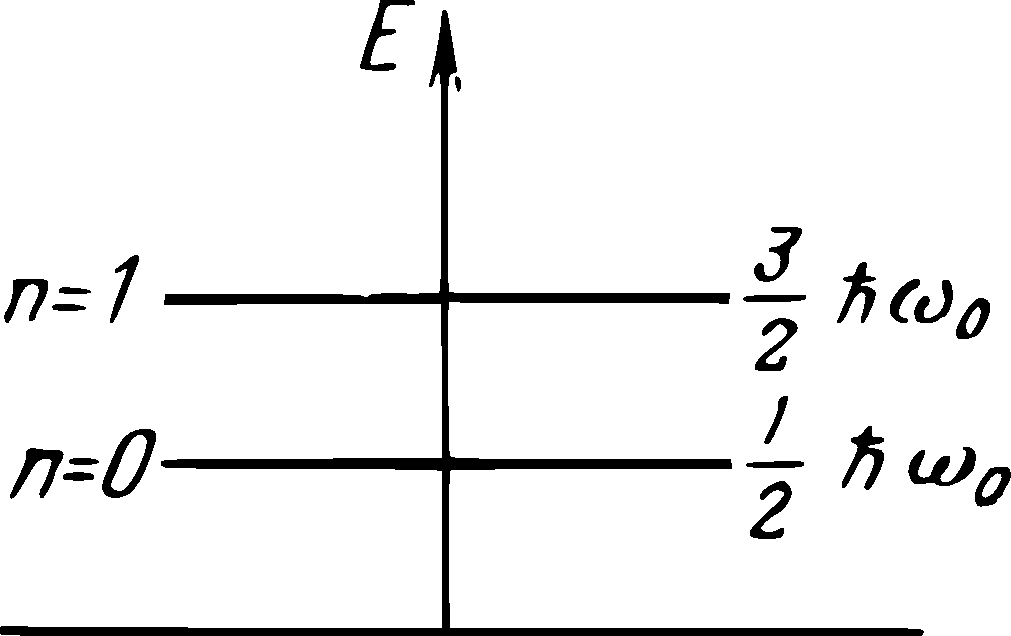
\includegraphics[width=0.8\textwidth]{figs/ch-38/fig-38-04.pdf}
\sidecaption{Energy levels of the oscillator.\zhcap{谐振子的能级。}\label{fig-38-04}}
\end{marginfigure}


\subsection{}\label{38.5.6} The minimum energy that can be had by a harmonic oscillator is called the \redem{zero-point energy} $E_{0}$:
\zhpar{谐振子所能具有的最小能量称为\redem{零点能} $E_{0}$，其表达式为：}
\begin{equation*}%
E_{0} =  \frac{h \nu_{0}}{2} = \frac{\hbar \omega_{0}}{2}  \quad \text{at } n = 0. 
\end{equation*}
In classical physics and in Planck's theory it was assumed that $E_{0} = 0$ (at $n = 0$). This means that the oscillator does not vibrate and is in a state of equilibrium. Atoms, as oscillators, should not, according to classical physics, execute any vibrations at the temperature of absolute zero $(T = 0)$. It has been proved in modern quantum mechanics, that the zero-point energy of a harmonic oscillator cannot be reduced however much it is cooled, even down to absolute zero \ssect{11.8.4}. Zero-point energy of the oscillator corresponds to its \redem{zero vibration}. 
\zhpar{在经典物理学和普朗克理论中，假定 $E_{0} = 0$（即 $n = 0$ 时）。这意味着振子不振动，处于平衡状态。按照经典物理学，原子作为振子，在绝对零度（$T = 0$）时不应有任何振动。现代量子力学证明，无论将谐振子冷却到多低，甚至冷却到绝对零度，其零点能都不能消除（\ssect{11.8.4}）。振子的零点能对应于其\redem{零振动}。}


In quantum mechanics, zero-point energy is a typical feature of any system of particles. At temperatures close to absolute zero, a substance is in a condensed state and its atoms (or molecules or ions) are dealt with as vibrating oscillators. Zero-point energy is the least amount of energy that a quantum oscillator should have in its lowest energy state (at
$n= 0$) in order to comply with the indeterminacy relation
\ssect{38.6.2}.
\zhpar{在量子力学中，零点能是各种粒子体系的典型特征。在接近绝对零度的温度下，物质处于凝聚态，其原子（或分子、离子）可视为作振动的振子。零点能是量子振子处于最低能态（$n= 0$）时所应具有的最小能量，以满足不确定关系（\ssect{38.6.2}）。}


\begin{marginfigure}%[-3cm] 
\centering
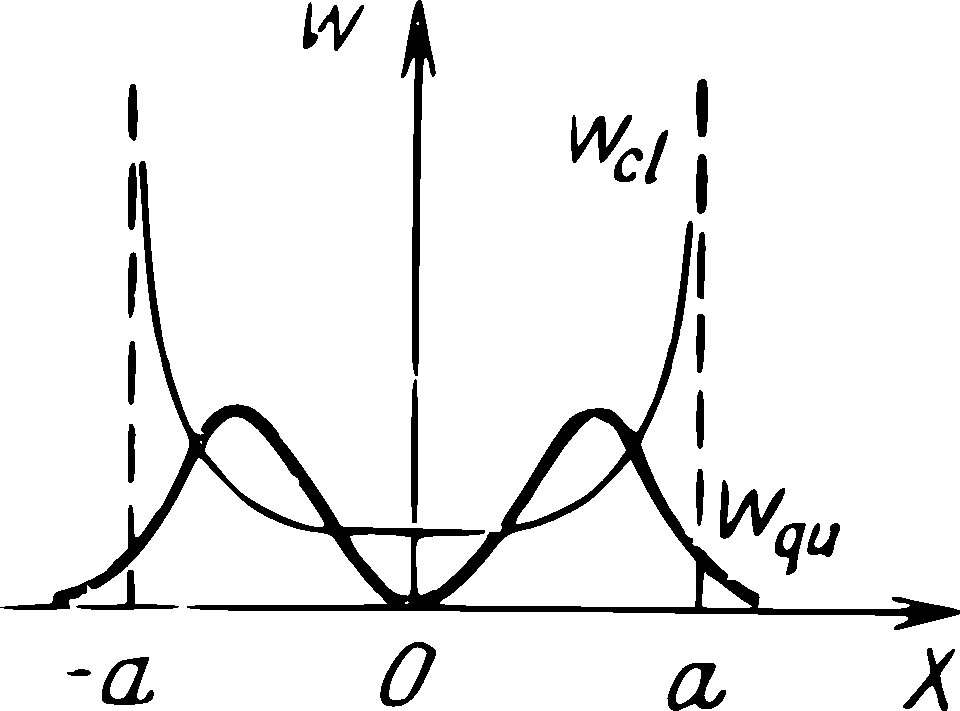
\includegraphics[width=0.8\textwidth]{figs/ch-38/fig-38-05.pdf}
\sidecaption{Comparison of probability density for classical and quantum cases for the linear harmonic oscillator for $n =1$.\zhcap{线性谐振子在 $n =1$ 时经典与量子概率密度的比较。}\label{fig-38-05}}
\end{marginfigure}

\subsection{}\label{38.5.7} The probability of find­ing a quantum linear harmonic oscillator on the $OX$ axis in
the region from $x$ to $x + \dd x$ is
\zhpar{量子线性谐振子在 $OX$ 轴上从 $x$ 到 $x + \dd x$ 区间内被发现的概率为：}
\begin{equation*}%
w_{qu} (x) \dd x = \abs{\psi_{}n (x)}^{2} \dd x.
\end{equation*}
Compared in \figr{fig-38-05} are the quantum probability density at $n - 1$ and the classical probability density $w_{cl} (x)$. The existence of nonzero values of $w_{qu}( x)$ beyond the limits of the classically allowed region  $\abs{x} \geqslant a$ is explained by the feasibility of the passing of particles possessing wavelike properties through a potential barrier \ssect{38.7.2}.
\zhpar{\figr{fig-38-05}比较了 $n - 1$ 时的量子概率密度与经典概率密度 $w_{cl} (x)$。量子概率 $w_{qu}( x)$ 在经典允许区域 $\abs{x} \geqslant a$ 之外不为零，这可以用具有波动性质的粒子能够穿过势垒来解释（\ssect{38.7.2}）。}

\subsection{}\label{38.5.8} As the number $n$ is increased, the probability distribution curve $\abs{\psi}^{2}$, illustrated in \figr{fig-38-06} for $n = 10$, becomes more and more like the classical probability distribution curve \figr{fig-38-03}. This agrees with Bohr's correspondence principle \ssect{38.4.4}.
\zhpar{随着 $n$ 增大，$n = 10$ 时的概率分布曲线 $\abs{\psi}^{2}$（如\figr{fig-38-06}所示）越来越接近经典的概率分布曲线（见\figr{fig-38-03}）。这与玻尔对应原理相一致（\ssect{38.4.4}）。}

\begin{figure}%[-3cm]
\centering
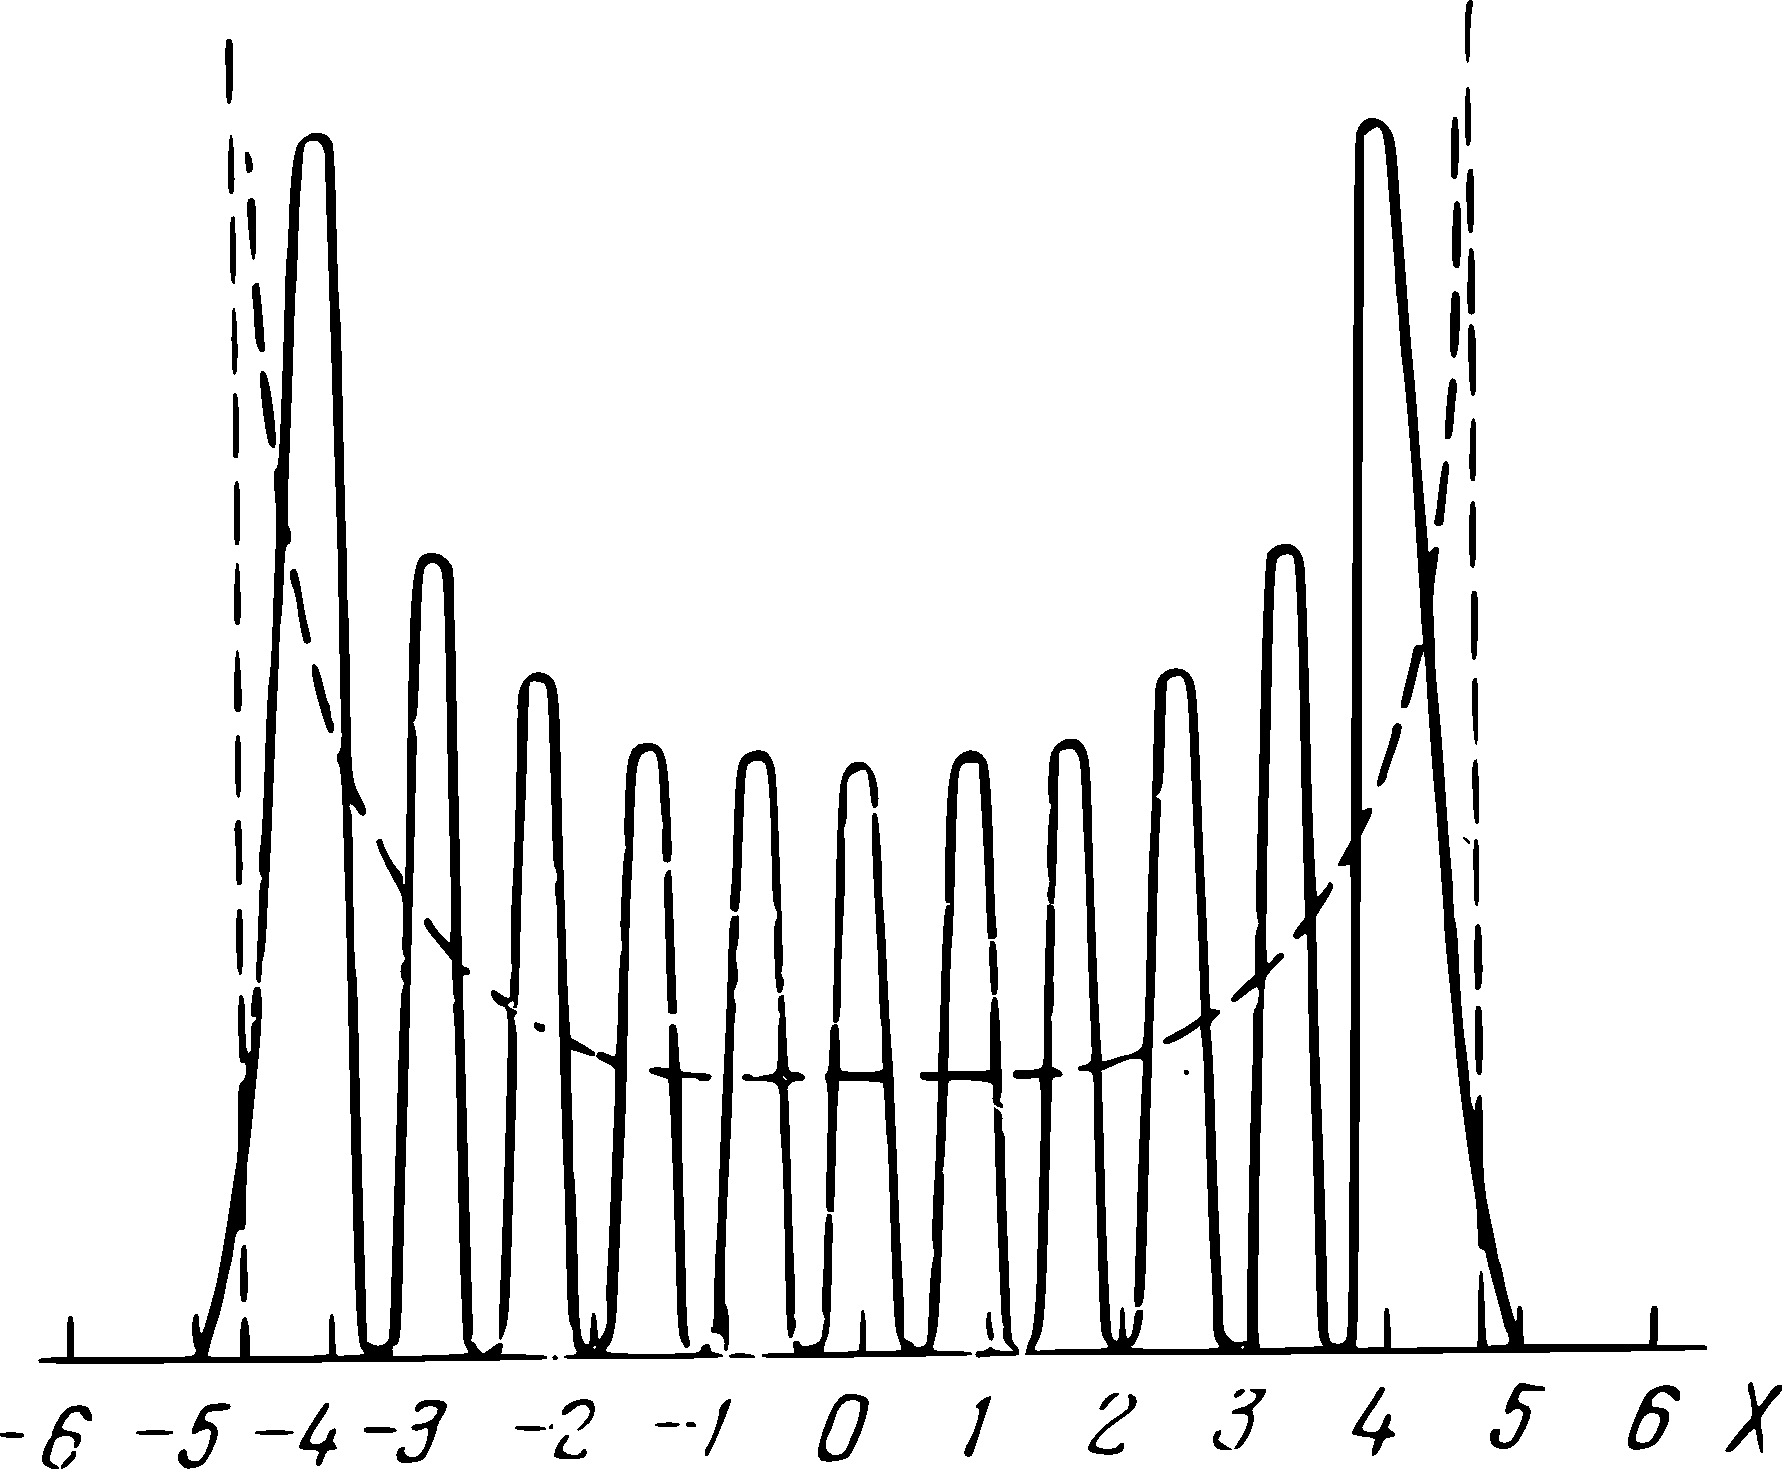
\includegraphics[width=0.8\textwidth]{figs/ch-38/fig-38-06.pdf}
\sidecaption{Comparison of probability density for classical and quantum cases for the linear harmonic oscillator for $n =10$.\zhcap{线性谐振子在 $n =10$ 时经典与量子概率密度的比较。}\label{fig-38-06}}
\end{figure}


\subsection{}\label{38.5.9} Making use of the eigenfunctions of the energy of a linear harmonic oscillator, the average energy $\expval{E}$ of such an oscillator can be calculated:
\zhpar{利用线性谐振子能量的本征函数，可以计算该振子的平均能量 $\expval{E}$：}
\begin{equation*}%
\expval{E} = \frac{\hbar \omega_{0}}{2} + \frac{\hbar \omega_{0}}{\exp (\hbar \omega_{0}/kT) -1} = \frac{\hbar \omega_{0}}{2} + \expval{E_{1}}.
\end{equation*}
Accurate to within zero-point energy, $\expval{E}$ is expressed by the term $\expval{E_{1}}$, which was obtained by Planck in developing his theory of the thermal radiation of a blackbody. Graphically, this term is represented in \figr{fig-38-07}, at $T = \text{const.}$, as a function of the frequency. It is evident that the greatest contribution to $\expval{E_{1}}$ is made by vibrations with low frequencies, corresponding to long wavelengths.
\zhpar{除零点能外，$\expval{E}$ 由项 $\expval{E_{1}}$ 给出，该项是普朗克在建立黑体热辐射理论时得到的。在 $T = \text{const.}$ 时，该项作为频率的函数，其图像如\figr{fig-38-07}所示。显然，对 $\expval{E_{1}}$ 贡献最大的是低频振动，即对应长波长的振动。}

\begin{marginfigure}%[-3cm] 
\centering
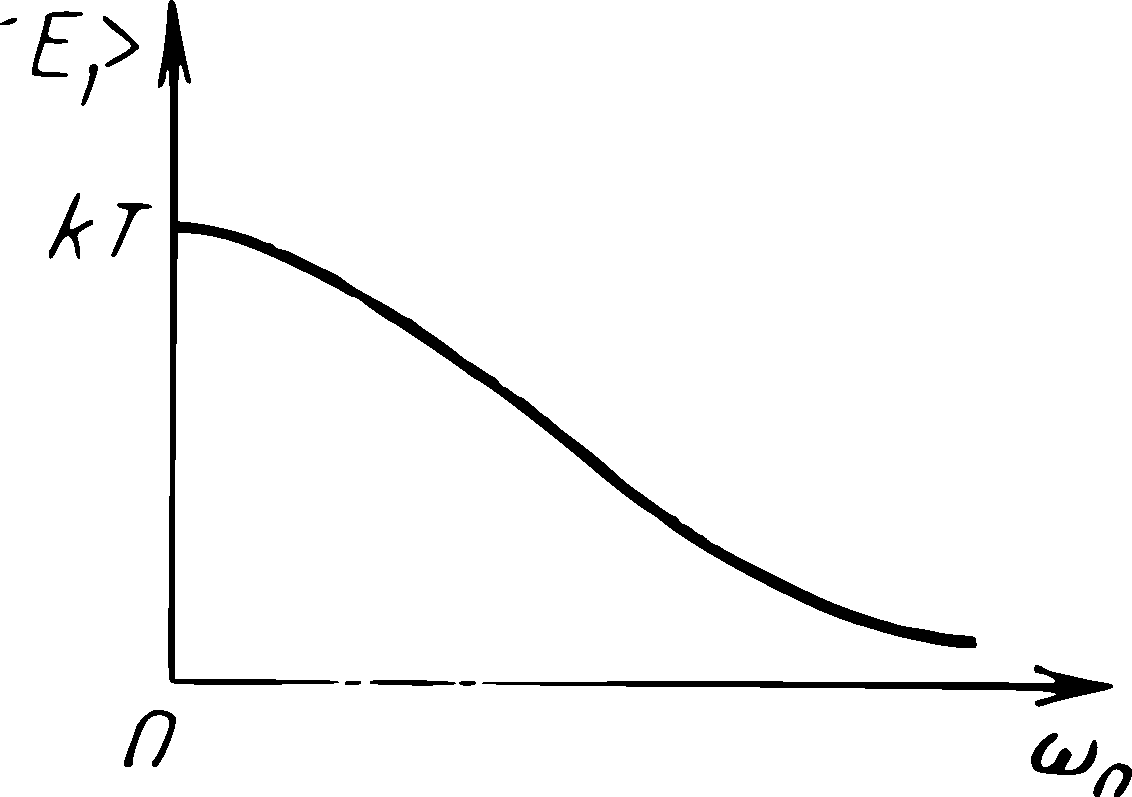
\includegraphics[width=0.8\textwidth]{figs/ch-38/fig-38-07.pdf}
\sidecaption{Expectation value (average energy) of linear harmonic oscillator.\zhcap{线性谐振子的期望值（平均能量）。}\label{fig-38-07}}
\end{marginfigure}

At a high temperature $(kT \gg \hbar \omega_{0})$
\zhpar{在高温情形（$kT \gg \hbar \omega_{0}$）下，有：}
\begin{equation*}%
\expval{E_{1}} = \frac{\hbar \omega_{0}}{1 + \dfrac{\hbar \omega_{0}}{kT} - 1} = kT.
\end{equation*}
This result coincides with that obtained from the principle of
equipartition of energy \ssect{10.6.4}.
\zhpar{这一结果与由能量均分原理（\ssect{10.6.4}）得到的结果相一致。}

\section{Heisenberg Indeterminacy Principle}
\label{sec-38.6} 
\zhtitle{海森伯不确定关系}


\subsection{}\label{38.6.1} The wavelike properties of microparticles \ssect{38.1.4} introduce limitations into the possibility of applying the concepts of coordinates and momentum in their classical form to such particles.
Limitations also exist in classical physics in the application of certain concepts to definite items. It is of no meaning, for instance, to apply the idea of temperature to a single molecule; the concept of point localization (location at a certain point) is inapplicable in determining the position of a wave in space, etc. But in classical mechanics, a definite value of the particle's coordinate corresponds to exact values of its velocity and momentum.
\zhpar{微观粒子的波动性（\ssect{38.1.4}）对于在经典形式下将坐标与动量概念应用于此类粒子的可能性施加了限制。经典物理中对某些概念的应用同样存在限制。例如，将温度概念应用于单个分子毫无意义；点定域（即位于空间某一点）的概念也无法用来确定波在空间中的位置，等等。但在经典力学中，粒子坐标的确定值对应于其速度和动量的确定值。}

In quantum mechanics there exist fundamental restrictions
in the possibility of simultaneously determining the
exact coordinate of a particle and its exact momentum. These
restrictions are associated with the wave-particle dualism of
the properties of microparticles \ssect{38.1.3}.
\zhpar{在量子力学中，同时精确确定粒子的坐标及其动量的可能性存在根本性的限制。这些限制与微观粒子性质的波粒二象性相关（\ssect{38.1.3}）。}

\subsection{}\label{38.6.2} The \redem{Heisenberg indeterminacy relations} are the inequalities
\zhpar{\redem{海森伯不确定关系}为如下不等式：}
\begin{align*}%
\Delta x \times \Delta p_{x} & \geqslant \frac{\hbar}{2},\\
\Delta y \times \Delta p_{y} & \geqslant \frac{\hbar}{2},\\
\Delta z \times \Delta p_{z} & \geqslant \frac{\hbar}{2}.
\end{align*}
Here $\Delta x$, $\Delta y$ and $\Delta z$ are the ranges of the coordinates within which a particle, described by a de Broglie wave \ssect{38.1.4}, may be localized if the projections of its momentum along the coordinate axes are within the ranges $\Delta p_{x}$, $\Delta p_{y}$ and $\Delta p_{z}$. The Heisenberg relations indicate that the coordinates $x$, $y$, and $z$ of the particle and the projections $p_{x}$, $p_{y}$ and $p_{z}$ of its momentum on the corresponding axes cannot simultaneously have values exactly equal to $x$ and $p_{x}$, $y$ and $p_{y}$, and $z$ and $p_{z}$. These physical
quantities can have values given to an accuracy determined by
the Heisenberg relations. The more accurately the position of
the particle is determined, i.e. the smaller the values of $\Delta x$, $\Delta y$ and $\Delta z$, the less accurately the values are determined for the projections of its momentum (i.e. the greater are $\Delta p_{x}$, $\Delta p_{y}$ and $\Delta p_{z}$). If the position of the particle along the $OX$ axis is exactly determined and $\Delta x = 0$, then $\Delta p_{x} = \infty$ and the value of the projection $p_{x}$ of the momentum on this axis becomes entirely indeterminate.
\zhpar{式中 $\Delta x$、$\Delta y$ 和 $\Delta z$ 为粒子坐标的取值范围：若粒子动量沿坐标轴的投影分别处于 $\Delta p_{x}$、$\Delta p_{y}$ 和 $\Delta p_{z}$ 的范围内，则由德布罗意波描述的粒子（\ssect{38.1.4}）可能被定域在这些坐标范围之内。海森伯关系表明，粒子的坐标 $x$、$y$、$z$ 及其动量在相应坐标轴上的投影 $p_{x}$、$p_{y}$、$p_{z}$ 不能同时精确地等于 $x$ 和 $p_{x}$、$y$ 和 $p_{y}$、$z$ 和 $p_{z}$ 的值。这些物理量只能在海森伯关系所决定的精度范围内取值。粒子位置确定得越精确，即 $\Delta x$、$\Delta y$ 和 $\Delta z$ 越小，其动量投影的数值就越不精确（即 $\Delta p_{x}$、$\Delta p_{y}$ 和 $\Delta p_{z}$ 越大）。若粒子沿 $OX$ 轴的位置被精确确定，即 $\Delta x = 0$，则 $\Delta p_{x} = \infty$，动量在该轴上的投影 $p_{x}$ 就变得完全不确定。}

\subsection{}\label{58.6.3} The indeterminacy relations put definite restrictions in quantum mechanics on the feasibility of describing the motion of a particle along a certain path. 
\zhpar{不确定关系使量子力学中描述粒子沿某一轨迹运动的可能性受到确定的限制。}

In classical theory each point of the path of a particle has definite coordinates $x$, $y$, and $z$ and the particle has a definite momentum $\vb{p}$ with projections $p_{x}$, $p_{y}$ and $p_{z}$ along the coordinate axes. This is realized in quantum mechanics only in cases when the particle travels in a macroscopic region of space (for instance, the particle may leave a trace on a photographic plate or on the screen of an oscillograph). If, for example, the position of an electron is fixed with an accuracy determined by the linear dimensions of a grain of photographic emulsion, subject to the (effect of the electron, then $\Delta x \approx \SI{d-6}{\meter}$. This corresponds to an indeterminacy in the momentum equal to Apx $\Delta p_{x} \geqslant \hbar/2 \Delta x \approx \SI{d-28}{\kilo\gram\meter\per\second}$ and in the velocity equal to $\Delta v_{x} = \Delta p_{x}/m \approx \SI{d2}{\meter\per\second}$. This indeterminacy at electron velocities of the order of $\num{d6}$ to $\SI{d7}{\meter\per\second}$, enables us to assume that the electron is travelling along a definite path with an exact velocity specified at each point of this path.
\zhpar{在经典理论中，粒子轨迹上的每一点都具有确定的坐标 $x$、$y$、$z$，粒子也具有确定的动量 $\vb{p}$，其在各坐标轴上的投影为 $p_{x}$、$p_{y}$ 和 $p_{z}$。量子力学只有在粒子于宏观空间区域内运动的情形下才能实现这一图像（例如粒子可在照相底片或示波器屏幕上留下痕迹）。若电子位置的确定精度由照相乳胶颗粒的线度所决定，则 $\Delta x \approx \SI{d-6}{\meter}$，相应的动量不确定量为 $\Delta p_{x} \geqslant \hbar/2 \Delta x \approx \SI{d-28}{\kilo\gram\meter\per\second}$，速度不确定量为 $\Delta v_{x} = \Delta p_{x}/m \approx \SI{d2}{\meter\per\second}$。在电子速度约为 $\num{d6}$ 至 $\SI{d7}{\meter\per\second}$ 的情形下，这种不确定性使我们能够假定：电子沿着确定的轨迹运动，并在该轨迹的每一点都具有确定的速度。}

\subsection{}\label{38.6.4} If the particle is travelling in a microscopic region of space, the indeterminacy relations substantially affect the nature of its motion. For example, the position of an electron travelling in an atom can be determined with an accuracy to the dimensions of the atom, i.e. $\Delta x  \approx \SI{d-10}{\meter}$. But the indeterminacy of the electron's velocity $\Delta v_{x}$, in this case, is found to be of the same order of magnitude as the velocity itself: $\Delta v_{x}  \approx \SI{d6}{\meter\per\second} \approx v$. The path of an electron in an atom with the exact velocity specified at each point does not have the meaning it has in classical mechanics \ssect{1.2.3}. This by no means indicates that the indeterminacy principle places fundamental limitations on our knowledge of the microcosm. It only indicates the limited applicability of the concepts of classical physics to the region of the microcosm.
\zhpar{若粒子在微观区域内运动，不确定关系会实质性地影响其运动性质。例如，原子中运动的电子，其位置可以确定到原子线度的精度，即 $\Delta x \approx \SI{d-10}{\meter}$。但在这种情形下，电子速度的不确定量 $\Delta v_{x}$ 与速度本身为同一数量级：$\Delta v_{x} \approx \SI{d6}{\meter\per\second} \approx v$。因此，原子中每一点都具有确定速度的电子轨迹，已不再具有经典力学中的意义（\ssect{1.2.3}）。这绝不意味着不确定原理对人们认识微观世界施加了根本性的限制，它只表明经典物理概念在微观世界中的适用范围是有限的。}

\subsection{}\label{38.6.5} No restrictions are made by the indeterminacy principle with respect to the feasibility of applying the conception of the coordinate and momentum of a macroscopic body in the classical sense. The wave properties of such bodies are not manifested in any way \ssect{38.1.6} and, consequently, the indeterminacy relations are not applied to them.
\zhpar{不确定原理对于在经典意义上将坐标和动量概念应用于宏观物体，不施加任何限制。这类物体的波动性质完全不表现出来（\ssect{38.1.6}），因此不确定关系不适用于它们。}

\subsection{}\label{38.6.6} The indeterminacy relations for energy $E$ and time $t$ are
\zhpar{能量 $E$ 与时间 $t$ 之间的不确定关系为：}
\begin{equation*}%
\Delta E \times \Delta t  \geqslant \hbar.
\end{equation*}
where $\Delta E$ is the indeterminacy of the energy of a particle, which is in a state with the energy $E$ during the length of time $\Delta t$. The longer a particle is in the given state, the more accurately its energy in this state can be determined.
\zhpar{式中 $\Delta E$ 为粒子处于能量为 $E$ 的状态期间其能量的不确定量，该状态持续的时间为 $\Delta t$。粒子处于给定状态的时间越长，就越能精确地确定其在该状态下的能量。}

\subsection{}\label{38.6.7} \redem{Measurement} is the process of interaction of an instrument with the item being investigated as a result of which certain information is obtained on the properties of the item. This process proceeds in space and time and is an objective process.
\zhpar{\redem{测量}是测量仪器与被研究对象相互作用的过程，通过这一过程获得关于被研究对象性质的某些信息。该过程在空间和时间中进行，是一个客观过程。}

The interaction between the measuring instrument and the item
being measured essentially differs for microscopic and macroscopic items. In the latter case, the measuring process is described with more or less accuracy by the laws of classical physics, and the instrument has no effect on the item being measured that cannot be accurately taken into account in the terms and con­ cepts of classical physics or reduced to as small a value as desired.
\zhpar{测量仪器与被测对象之间的相互作用，对于微观对象与宏观对象本质上是不同的。对于后者，测量过程或多或少可以用经典物理的规律精确描述；仪器对被测对象的作用，要么能用经典物理的术语和概念准确地加以考虑，要么可以任意减小到足够小的程度。}

In quantum mechanics, owing to the objectively existing duality of the properties of microscopic items \ssect{38.1.3}, the measuring process is inevitably associated with substantial effects of the instrument on the course of the phenomenon being investigated.
\zhpar{在量子力学中，由于微观对象的性质客观上具有二象性（\ssect{38.1.3}），测量过程必然伴随着仪器对所研究现象进程的实质性影响。}

For example, to determine the position of the electron it
must be ``illuminated'' by light of the highest possible frequency. As a result of the collision between the photon and the electron, the momentum $p_{x}$ of the latter is changed by an amount determined by the indeterminacy relation: $\Delta p_{x} \geqslant \hbar/2\Delta x$ \ssect{38.6.2}. This
effect on the item being measured cannot be considered small
or inessential because the state of the item is changed. This
change is such that as a result of measurement, definite classical characteristics of a particle, for instance, its momentum, are found to be specified only within the limits restricted by the indeterminacy relations.
\zhpar{例如，为了确定电子的位置，必须用频率尽可能高的光对其进行“照明”。光子与电子碰撞的结果，使电子的动量 $p_{x}$ 改变了一个量，该量由不确定关系 $\Delta p_{x} \geqslant \hbar/2\Delta x$（\ssect{38.6.2}）决定。这种对被测对象的作用不能视为小量或可以忽略，因为被测对象的状态已经发生了改变。这种改变使得：经测量后，粒子的某些确定的经典特征（例如其动量）只能被限定在不确定关系所允许的范围之内。}

\section{Tunnel Effect}
\label{sec-38.7} 
\zhtitle{隧道效应}

\begin{marginfigure}%[-3cm]
\centering
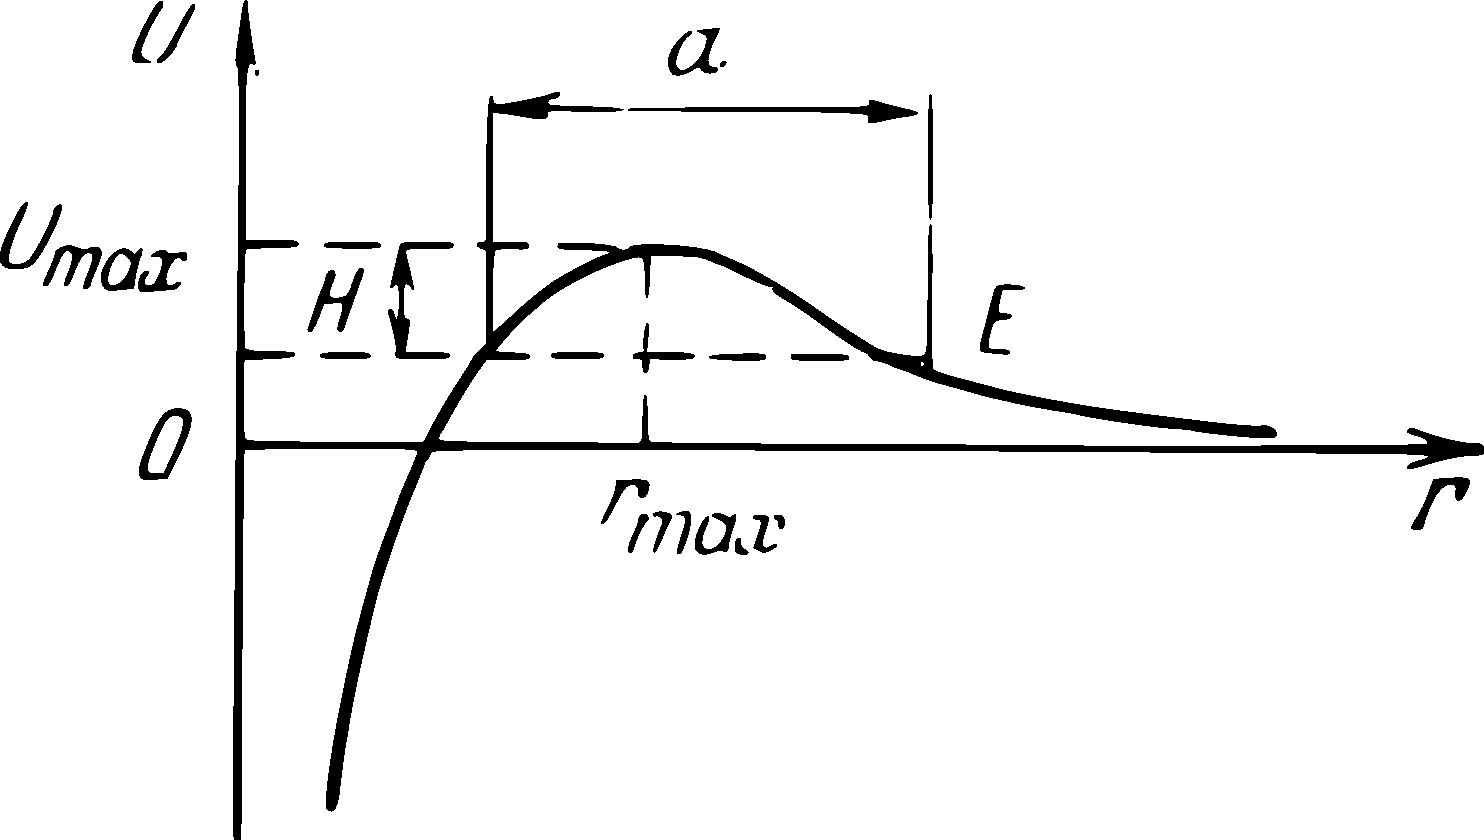
\includegraphics[width=\textwidth]{figs/ch-38/fig-38-08.pdf}
\sidecaption{Potential well of the form $U = U (r)$.\zhcap{$U = U (r)$ 形式的势阱。}\label{fig-38-08}}
\end{marginfigure}


\subsection{}\label{38.7.1} Potential wells in which particles are located may be of much more complicated shape than those dealt with in Section~\ref{sec-38.4}. If the potential energy of the particle is of the form $U = U (r)$, as shown in \figr{fig-38-08}, the particle moves in a field of forces that can be represented in the form of a \redem{potential barrier}. This means that the forces act on the particle in a certain limited region of space. Outside of this region the particles move as free ones.
\zhpar{粒子所处的势阱，其形状可能比\ssect{38.4}中所讨论的势阱复杂得多。若粒子的势能具有 $U = U (r)$ 的形式（如\figr{fig-38-08}所示），则粒子在一个可以表示为\redem{势垒}的力场中运动。这意味着，力只在空间中某一有限区域内作用于粒子；在该区域之外，粒子如同自由粒子一样运动。}

The height $H$ of the barrier and its width $a$ for a given particle depend upon the energy $E$ of the particle. In order for a particle to get out of a potential well or to enter it from outside, it is necessary, according to classical mechanics, to impart energy to the particle equal to or greater than $\abs{U_{max} - E} = H$.
\zhpar{势垒的高度 $H$ 及其宽度 $a$ 取决于粒子的能量 $E$。按照经典力学，粒子要逸出势阱或从外部进入势阱，必须赋予粒子不小于 $\abs{U_{max} - E} = H$ 的能量。}

\subsection{}\label{38.7.2} The \redem{tunnel effect} is the passing (``leaking'') of particles through potential barriers. The tunnel effect is a quantum-mechanical one and is due to the wavelike properties of the particles \ssect{38.1.3}.
\zhpar{\redem{隧道效应}是粒子穿过（“泄漏”过）势垒的现象。隧道效应是一种量子力学效应，源于粒子的波动性质（\ssect{38.1.3}）。}

The \redem{penetrability (penetrability factor)} $D$ of a potential barrier is the quantity
\zhpar{势垒的\redem{穿透系数}（\redem{穿透因子}）$D$ 定义为：}
\begin{equation*}%
D = \frac{I_{tran}}{I_{inc}},
\end{equation*}
where $I_{tran}$ is the intensity \ssect{30.3.6} of de Broglie waves passing through the potential barrier, and $I_{inc}$ is the intensity of the waves incident on the barrier.
\zhpar{式中 $I_{tran}$ 为穿过势垒的德布罗意波的强度（\ssect{30.3.6}），$I_{inc}$ 为入射到势垒上的波的强度。}

\begin{marginfigure}%[-3cm]
\centering
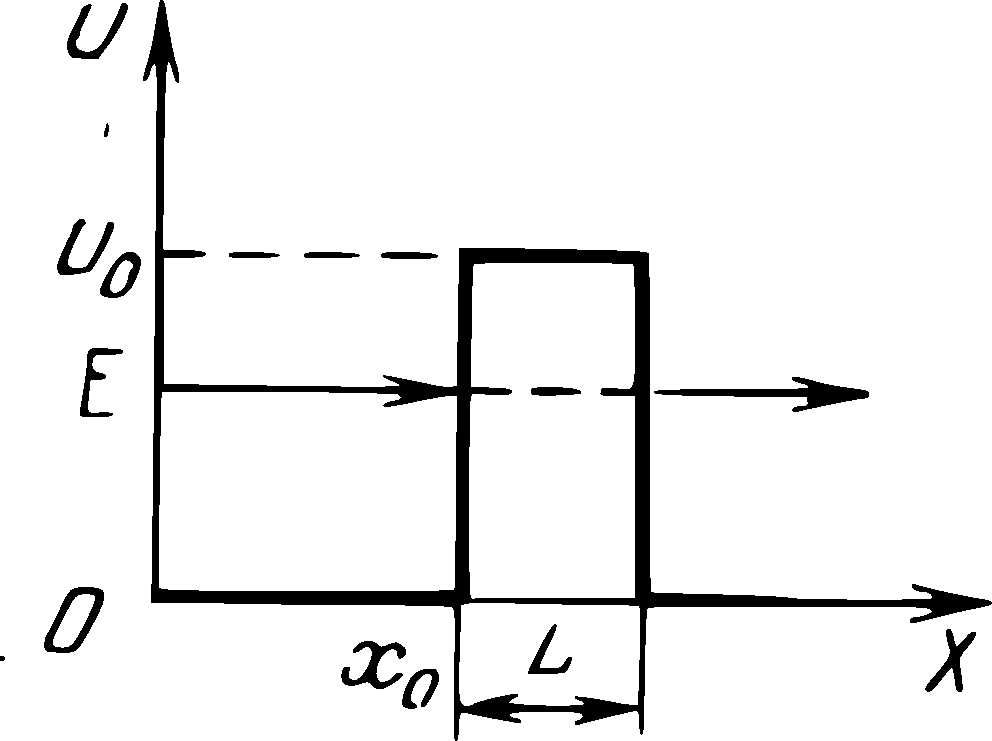
\includegraphics[width=\textwidth]{figs/ch-38/fig-38-09.pdf}
\sidecaption{A rectangular potential well with height $U_{0}$ and width $L$.\zhcap{高为 $U_{0}$、宽为 $L$ 的矩形势阱。}\label{fig-38-09}}
\end{marginfigure}

The penetrability of a rectangular potential barrier of the height $U_{0}$ and width $L$ (\figr{fig-38-09}) is
\zhpar{高度为 $U_{0}$、宽度为 $L$ 的矩形势垒（见\figr{fig-38-09}）的穿透系数为：}
\begin{equation*}%
D = D_{0} \exp \left[ - \frac{2}{\hbar}  \sqrt{2 m (U_{0} - E)} \, L \right],
\end{equation*}
where $m$ is the mass of the particle, and $E$ is its energy.
For a potential barrier of complex shape
\zhpar{式中 $m$ 为粒子的质量，$E$ 为其能量。对于形状复杂的势垒，穿透系数为：}
\begin{equation*}%
D = D_{0} \exp \left[ - \frac{2}{\hbar} \int_{x_{1}}^{x_{2}}  \sqrt{2 m (U_{0} - E)} \dd x \right],
\end{equation*}
where $x_{1}$ and $x_{2}$ are the coordinates of the points at the beginning and end of the potential barrier $U (x)$ for a given value $E$ of the total energy (\figr{fig-38-10}. In these formulas $D_{0}$ is a constant factor close to unity.
\zhpar{式中 $x_{1}$ 和 $x_{2}$ 分别为对应于给定总能量 $E$ 时，势垒 $U (x)$ 起点和终点的坐标（见\figr{fig-38-10}）。在这些公式中，$D_{0}$ 为接近于 1 的常数因子。}

\begin{marginfigure}%[-3cm]
\centering
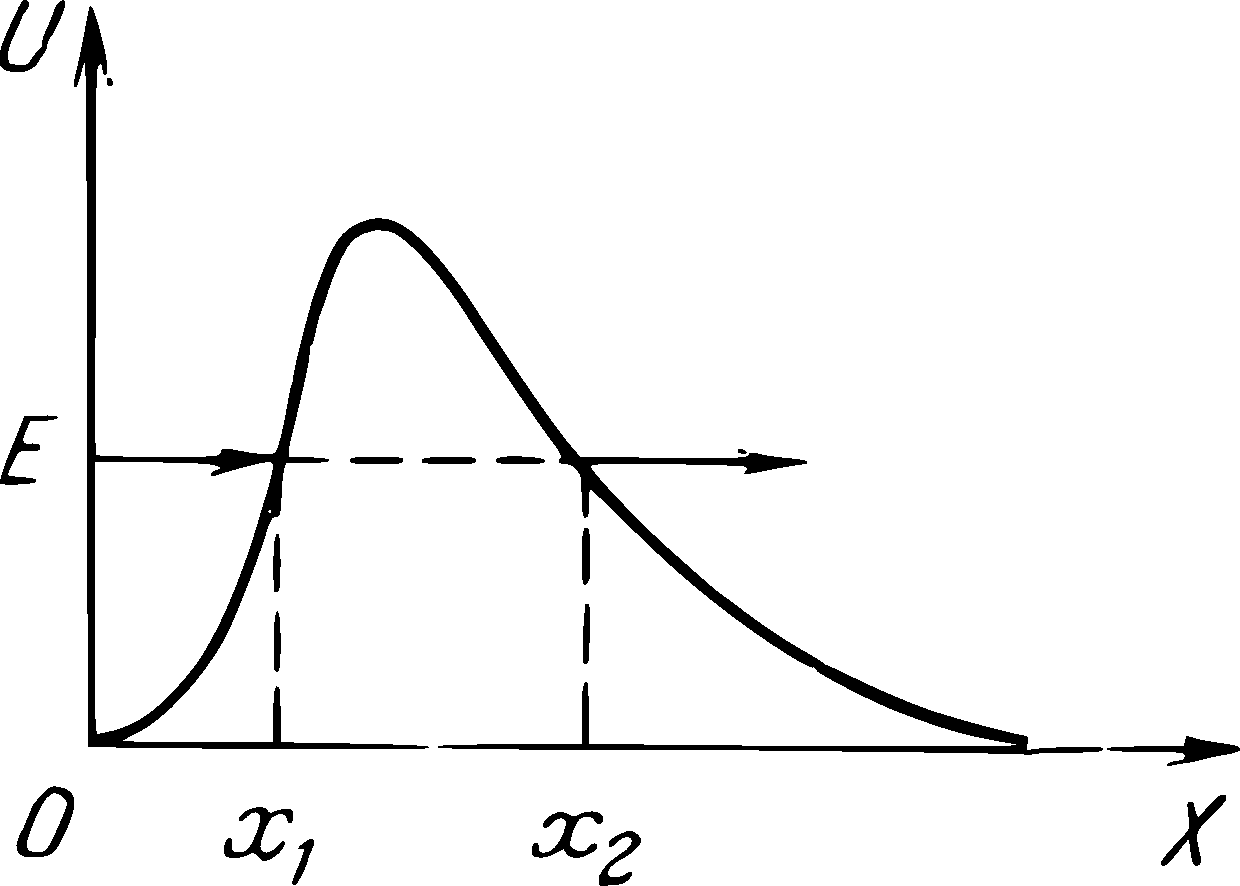
\includegraphics[width=\textwidth]{figs/ch-38/fig-38-10.pdf}
\sidecaption{A potential well of a complex shape.\zhcap{形状复杂的势阱。}\label{fig-38-10}}
\end{marginfigure}

\subsection{}\label{38.7.3} The tunnel effect plays an important role when the penetrability is not too low. This occurs in the cases when the linear dimensions of the potential barrier are commensurable with atomic dimensions. For example, at $U_{0} - E = \SI{10}{\electronvolt}$ for an
electron $(m \approx \SI{d-30}{\kilo\gram})$ and $L = \SI{d-10}{\meter}$, we obtain $D \approx 1/e$.
\zhpar{隧道效应在穿透系数不太小时起重要作用。当势垒的线度与原子线度相当时，即属于这种情形。例如，对于质量 $m \approx \SI{d-30}{\kilo\gram}$ 的电子，当 $U_{0} - E = \SI{10}{\electronvolt}$、$L = \SI{d-10}{\meter}$ 时，可得 $D \approx 1/e$。}

Under the same conditions, excepting that $L = \SI{d-2}{\meter}$, $D \approx \exp (\num{d-8})$. The penetrability of the barrier decreases with an increase in the mass of the particle and in the difference $U_{0} - E$.
\zhpar{在其他条件相同、仅将 $L$ 改为 \SI{d-2}{\meter} 的情形下，$D \approx \exp (\num{d-8})$。势垒的穿透系数随粒子质量以及差值 $U_{0} - E$ 的增大而减小。}

\subsection{}\label{38.7.4} The \redem{paradox of the tunnel effect} is that the passing of a particle through the potential barrier enables it to be found in a region that is forbidden from the classical point of view. In this region the potential energy of the particle exceeds its total energy; its kinetic energy is negative and, consequently, the velocity (momentum) of the particle becomes an imaginary quantity.
\zhpar{\redem{隧道效应佯谬}是指：粒子穿过势垒后，可能出现在经典观点下被禁止的区域中。在该区域内，粒子的势能超过其总能量，动能为负，因而粒子的速度（动量）成为虚数。}

Actually no such paradox exists. The tunnel effect is a purely
quantum-mechanical phenomenon and here an unexpected difficulty arises, from the classical point of view, in representing the total energy E in the form of the sum of the kinetic and potential energies: $E = p^{2}/2m + U (x)$. Owing to the fact
that the indeterminacy relation \ssect{38.6.2} excludes the possibility of simultaneously specifying definite values, to any degree of accuracy, for the coordinate x and momentum p of a particle, it is found to be inadmissible in quantum mechanics to represent the total energy as the sum of two exactly definite parts: the kinetic $p^{2}/2m$ and potential $U (x)$ energies. If the coordinate $x$ of the particle is fixed in the region $\Delta x$ and its potential energy $U (x)$ is determined with sufficient accuracy, then the indeterminacy $\Delta p$ introduced into the value of the particle's momentum $(\Delta p \approx \hbar/ A)$ excludes the possibility of specifying the exact value of the kinetic energy $p^{2}/2m$ of the particle.
\zhpar{实际上并不存在这种佯谬。隧道效应是纯粹的量子力学现象。从经典观点来看，这里出现了一个意想不到的困难：难以将总能量 $E$ 表示为动能与势能之和 $E = p^{2}/2m + U (x)$。由于不确定关系（\ssect{38.6.2}）不允许同时以任意精度确定粒子坐标 $x$ 和动量 $p$ 的确定值，因此在量子力学中，把总能量表示为两个确定部分——动能 $p^{2}/2m$ 与势能 $U (x)$ 之和——是不允许的。若粒子坐标 $x$ 被限定在区域 $\Delta x$ 内，且其势能 $U (x)$ 被足够精确地确定，则由此引入的粒子动量不确定量 $\Delta p$（$\Delta p \approx \hbar/ A$）就排除了精确确定粒子动能 $p^{2}/2m$ 的可能性。}

Consequently, the previous value of the particle's total energy $E$ cannot be specified either. It is found, in this case, that the change in the kinetic energy AE, caused by fixing the particle's coordinate, exceeds the difference between the barrier height $U_{0}$ (\figr{fig-38-09}) and the total energy $E$ of the particle:
\zhpar{因此，粒子的总能量 $E$ 的原有数值也无法确定。在这种情形下，固定粒子坐标所引起的动能变化 $\Delta E_{k}$，超过了势垒高度 $U_{0}$（\figr{fig-38-09}）与粒子总能量 $E$ 之差：}
\begin{equation*}%
\Delta E_{k} > U_{0} - E.
\end{equation*}
Thus, $\Delta E_{k}$ exceeds the energy that the particle, inside the potential well, lacks to surmount the barrier ``in the classical way'' to get out of the well.
\zhpar{因此，$\Delta E_{k}$ 超过了粒子在势阱内以经典方式越过势垒、从而逸出势阱所缺少的能量。}

The role played by the tunnel effect in solid-state physics and
in the phenomenon of radioactive decay is dealt with in Sections \ssect{41.8.3} and \ssect{42.5.2}.
\zhpar{隧道效应在固体物理学和放射性衰变现象中所起的作用，将分别在\ssect{41.8.3}和\ssect{42.5.2}中讨论。}

% Local Variables:
% TeX-master: "handbook-physics"
% coding: utf-8
% End:
